\documentclass[12pt,a4paper]{report}

% ==========================================
% PACKAGES ET CONFIGURATION
% ==========================================
\usepackage[utf8]{inputenc}
\usepackage[T1]{fontenc}
\usepackage[french]{babel}
\usepackage{graphicx}
\usepackage[dvipsnames, table]{xcolor}

% Marges selon le modèle ISET :
% Haut: 2cm, Bas: 2cm, Gauche: 2cm, Droite: 2cm, Reliure: 0.5cm
% En-tête: 1.25cm, Pied de page: 1.25cm
\usepackage{geometry}
\geometry{
  a4paper,
  top=2cm,
  bottom=2cm,
  left=2.5cm,        % 2cm + 0.5cm reliure
  right=2cm,
  headsep=0.75cm,    % distance header -> texte
  headheight=1.25cm,
  footskip=1.25cm
}

% Police Times New Roman (selon modèle)
\usepackage{mathptmx}  % Times New Roman
\usepackage{setspace}
\onehalfspacing        % Interligne 1.5 ligne

% En-têtes et pieds de page
\usepackage{fancyhdr}
\pagestyle{fancy}
\fancyhf{}

% En-tête : titre du projet, taille 10pt, italique, souligné
\fancyhead[C]{%
  \fontsize{10}{12}\selectfont\itshape
  Farm AI : Système Intelligent de Gestion Agricole
}
\renewcommand{\headrulewidth}{0.5pt}

% Pied de page : ISET | N° page | Entreprise
\fancyfoot[L]{\fontsize{10}{12}\selectfont\itshape Iset Siliana}
\fancyfoot[C]{\fontsize{10}{12}\selectfont\itshape \thepage}
\fancyfoot[R]{\fontsize{10}{12}\selectfont\itshape Luniweb / Farm AI}
\renewcommand{\footrulewidth}{0.5pt}

% Style des titres selon le modèle ISET
\usepackage{titlesec}

% Titre 1 (chapter) : 20pt, Gras, minuscule, justifié, interligne 1.5
% Numérotation : Chapitre 1, Chapitre 2...
\titleformat{\chapter}[block]
  {\normalfont\fontsize{20}{24}\selectfont\bfseries}
  {Chapitre \thechapter\ :}
  {0.5em}
  {}
\titlespacing*{\chapter}{0pt}{12pt}{35pt}

% Titre 2 (section) : 16pt, Gras, minuscule, justifié
% Numérotation : 1. Titre ; 2. Titre...
\titleformat{\section}
  {\normalfont\fontsize{16}{20}\selectfont\bfseries}
  {\thesection.}
  {1em}
  {}
\titlespacing*{\section}{20pt}{20pt}{10pt}

% Titre 3 (subsection) : 14pt, Gras, minuscule, justifié
% Numérotation hiérarchique : 1.1, 1.2...
\titleformat{\subsection}
  {\normalfont\fontsize{14}{18}\selectfont\bfseries}
  {\thesubsection.}
  {1em}
  {}
\titlespacing*{\subsection}{10pt}{10pt}{5pt}

% Titre 4 (subsubsection) : 12pt, Gras, Italique, minuscule
% Numérotation en lettres : a. b. c.
\renewcommand{\thesubsubsection}{\alph{subsubsection}.}
\titleformat{\subsubsection}
  {\normalfont\fontsize{12}{16}\selectfont\bfseries\itshape}
  {\thesubsubsection}
  {1em}
  {}
\titlespacing*{\subsubsection}{5pt}{5pt}{0pt}

% Tableaux améliorés
\usepackage{booktabs}
\usepackage{array}
\usepackage{tabularx}

% Liens hypertexte
\usepackage{hyperref}
\hypersetup{
    colorlinks=true,
    linkcolor=black,
    filecolor=black,
    urlcolor=black,
    citecolor=black,
}

% Numérotation des figures et tableaux par chapitre
\usepackage{caption}
\captionsetup{font={it,normalsize}, justification=centering, labelsep=colon}

% Chaque chapitre commence sur une nouvelle page
\usepackage{etoolbox}
\pretocmd{\chapter}{\clearpage}{}{}

% ==========================================
% DÉBUT DU DOCUMENT
% ==========================================
\begin{document}

% Page de garde sans en-tête ni pied de page
\thispagestyle{empty}

% --------------------------------------------------------------
% PAGE DE GARDE (modèle ISET Siliana)
% --------------------------------------------------------------
\begin{titlepage}
  \begin{center}

    % ---- En-tête institutionnel ----
    {\large \textbf{REPUBLIQUE TUNISIENNE}} \\[2pt]
    {\normalsize \textbf{MINISTERE DE L'ENSEIGNEMENT SUPERIEUR ET DE LA RECHERCHE SCIENTIFIQUE}} \\[2pt]
    {\normalsize \textbf{DIRECTION GENERALE DES ETUDES TECHNOLOGIQUES}} \\[0.8cm]

    % Logos (décommentez et adaptez si disponibles)
    % \includegraphics[width=3cm]{logo_iset.png}

    {\Large \textbf{Institut Supérieur des Études Technologiques de Siliana}} \\[4pt]
    {\large \textbf{Département de Génie Électrique}}

    \vspace{1.5cm}
    \rule{\linewidth}{0.8pt}\\[0.4cm]
    {\Large \textbf{Projet de fin d'études}}\\[0.4cm]
    \rule{\linewidth}{0.8pt}

    \vspace{1cm}

    % Titre du projet (10 mots max)
    {\LARGE \textbf{Farm AI : Système intelligent de gestion agricole}}

    \vspace{2cm}

    % Bloc étudiant / encadrant
    \begin{minipage}{0.45\textwidth}
      \begin{flushleft}
        \emph{Élaboré par :}\\[4pt]
        \textbf{Mohamed Amine ABBASSI}
      \end{flushleft}
    \end{minipage}
    \hfill
    \begin{minipage}{0.45\textwidth}
      \begin{flushright}
        \emph{Encadré par :}\\[4pt]
        \textbf{Mme. Abir KHALDI} (Interne)\\
        \textbf{Mr. Rochdi ABID} (Externe)\\[8pt]
        \emph{Entreprise d'accueil :}\\[4pt]
        \textbf{Luniweb}
      \end{flushright}
    \end{minipage}

    \vfill

    {\large \textbf{Année universitaire : 2025 -- 2026}}\\[4pt]
    {\normalsize GE…/2025\_S2}

  \end{center}
\end{titlepage}

% --------------------------------------------------------------
% DÉDICACE
% --------------------------------------------------------------
\chapter*{Dédicace}
\addcontentsline{toc}{chapter}{Dédicace}
\textit{Je dédie ce travail à ma famille et à tous ceux qui m'ont soutenu...}

% --------------------------------------------------------------
% REMERCIEMENTS
% --------------------------------------------------------------
\chapter*{Remerciements}
\addcontentsline{toc}{chapter}{Remerciements}

\begin{itshape}
Au seuil de ce travail, nous souhaitons exprimer notre profonde gratitude à nos encadreurs,
Madame Abir KHALDI et Monsieur Rochdi ABID, pour la qualité de leur accompagnement, leur disponibilité
constante ainsi que la pertinence de leurs conseils tout au long de la réalisation de ce projet.
Leur encadrement a été d'une aide précieuse et déterminante.

Nous adressons également nos remerciements les plus respectueux aux membres du jury qui nous ont
fait l'honneur d'accepter d'évaluer ce travail.

Enfin, nous tenons à remercier toutes les personnes qui, de près ou de loin, ont contribué à notre
parcours et participé à notre développement personnel et académique.
\end{itshape}

% --------------------------------------------------------------
% TABLE DES MATIÈRES
% La pagination commence après la page de garde (donc ici dès le sommaire)
% --------------------------------------------------------------
\tableofcontents
\addcontentsline{toc}{chapter}{Table des matières}
\newpage

% Liste des figures (optionnel selon modèle)
\listoffigures
\addcontentsline{toc}{chapter}{Liste des figures}
\newpage

% Liste des tableaux (optionnel selon modèle)
\listoftables
\addcontentsline{toc}{chapter}{Liste des tableaux}
\newpage

% --------------------------------------------------------------
% INTRODUCTION GÉNÉRALE
% --------------------------------------------------------------
\chapter*{Introduction générale}
\addcontentsline{toc}{chapter}{Introduction générale}

\textbf{Contexte général :}
L'intégration de l'Intelligence Artificielle dans le domaine agricole représente aujourd'hui une
évolution majeure des pratiques de gestion. Dans un contexte où la traçabilité du personnel et la
sécurité des sites sont des enjeux critiques, les systèmes manuels montrent rapidement leurs limites.

\textbf{Objectifs du travail :}
Ce projet a pour objectif de concevoir et de développer la plateforme \textit{Farm AI}, un système
moderne visant à automatiser la gestion du personnel, le suivi des présences et la sécurité, grâce
à des technologies avancées de vision par ordinateur et une architecture web robuste.

\textbf{Organisation du rapport :}
Le présent rapport est structuré en quatre chapitres. Le premier chapitre présente le contexte et
l'état de l'art. Le deuxième chapitre aborde la spécification des besoins et la conception. Le
troisième chapitre décrit l'environnement et les choix techniques. Enfin, le quatrième chapitre
expose la réalisation et les tests effectués.

% --------------------------------------------------------------
% CHAPITRE 1 : Contexte et État de l'art
% --------------------------------------------------------------
\chapter{Contexte et État de l'art}

\section{Introduction}
Ce chapitre présente le contexte général du projet, la problématique liée à la gestion classique
des fermes, ainsi qu'une étude comparative des solutions existantes.

\section{Présentation du cadre du projet}

\subsection{Présentation de l'entreprise d'accueil}
Luniweb est une agence pluridisciplinaire spécialisée dans le numérique...

\subsection{Contexte général du projet}
La ferme connectée est au cœur de la transition technologique actuelle. Farm AI s'inscrit dans cette vision.

\section{Étude de l'existant et problématique}

\subsection{Critique de l'existant}
Les systèmes de pointage classiques et la gestion manuelle du personnel présentent de nombreuses
failles : erreurs de saisie, risques de fraude, absence de suivi en temps réel et coûts
administratifs élevés.

\subsection{Problématique}
Comment assurer un suivi précis, sécurisé et en temps réel des employés agricoles sans intervention
manuelle lourde ?

\section{État de l'art des solutions technologiques}

\subsection{L'intelligence artificielle et la vision par ordinateur}
Les réseaux de neurones convolutifs ont révolutionné la reconnaissance d'images.

\subsection{Les algorithmes de reconnaissance faciale}
Des librairies comme OpenCV et dlib permettent d'obtenir un haut niveau de précision.

\subsection{Les systèmes d'information et tableaux de bord interactifs}
Angular combiné avec un Backend Spring Boot offre la base parfaite pour afficher ces statistiques en temps réel.

\section{Solution proposée : le système Farm AI}
Farm AI combine l'IA et le Web pour un pointage entièrement automatisé.

\section{Conclusion}
Ce chapitre a permis d'identifier les lacunes des systèmes existants et de justifier le choix d'une
solution basée sur l'intelligence artificielle. Le chapitre suivant précisera les besoins fonctionnels
et non fonctionnels du système.

% --------------------------------------------------------------
% CHAPITRE 2 : Spécification des besoins et Conception
% --------------------------------------------------------------
\chapter{Spécification des besoins et Conception}

\section{Introduction}
Nous détaillons ici les fonctionnalités attendues du système Farm AI ainsi que la modélisation UML globale et les diagrammes des sprints.

\section{Spécification des besoins}

\subsection{Les besoins fonctionnels}
Le système doit répondre aux fonctionnalités suivantes :
\begin{itemize}
  \item \textbf{Gestion des employés :} Ajout, modification et enregistrement du \textit{Face ID}.
  \item \textbf{Reconnaissance faciale en temps réel :} Identification automatique via des caméras IP ou webcams.
  \item \textbf{Détection d'attributs :} Identification des couleurs de vêtements des employés.
  \item \textbf{Suivi et pointage :} Enregistrement automatique des entrées/sorties (Timeline).
  \item \textbf{Tableau de bord (Dashboard) :} Visualisation des statistiques analytiques.
\end{itemize}

\subsection{Les besoins non fonctionnels}
\begin{itemize}
  \item \textbf{Temps réel :} Traitement rapide du flux vidéo (latence minimale).
  \item \textbf{Sécurité :} Authentification robuste (JWT) et interface de connexion sécurisée.
  \item \textbf{Fiabilité :} Précision élevée du modèle d'IA (taux d'erreur acceptable).
\end{itemize}

\section{Conception globale et modélisation UML}

\subsection{Architecture globale du système}
Le système adopte une architecture micro-services séparant l'intelligence artificielle (FastAPI),
le backend logique (Spring Boot) et l'interface utilisateur (Angular).

\subsection{Diagramme des cas d'utilisation}
La figure \ref{fig:usecase} montre les différents acteurs interagissant avec le système Farm AI.

\begin{figure}[h]
  \centering
  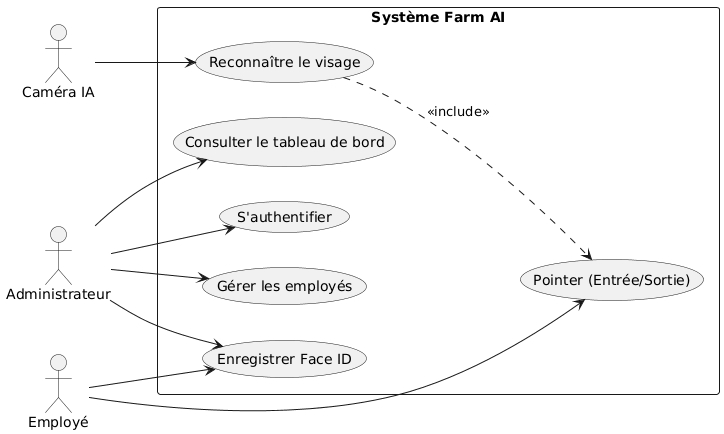
\includegraphics[width=0.8\textwidth]{usecase.png}
  \caption{Diagramme des cas d'utilisation du système Farm AI}
  \label{fig:usecase}
\end{figure}

\subsection{Diagrammes de séquences}

\subsubsection{Scénario d'authentification de l'administrateur}
La figure \ref{fig:seq_auth} illustre le processus de vérification des accès (Sprint 1).

\begin{figure}[h]
  \centering
  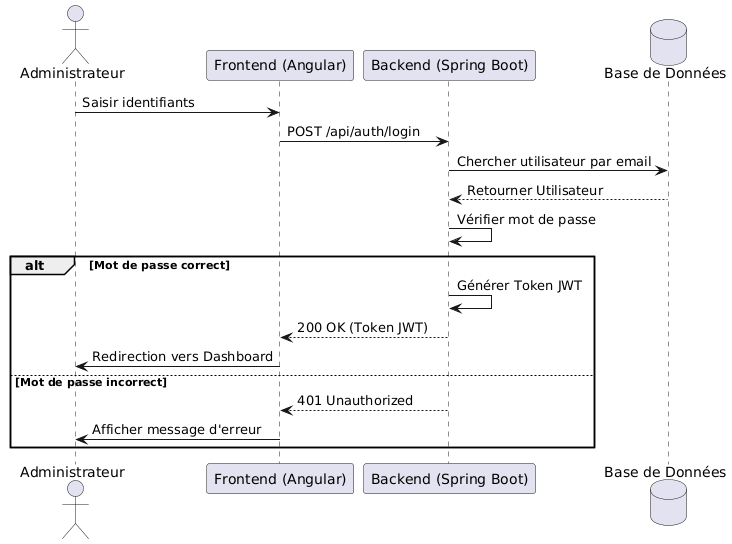
\includegraphics[width=0.9\textwidth]{seq_auth.png}
  \caption{Diagramme de séquence - Authentification}
  \label{fig:seq_auth}
\end{figure}

\subsubsection{Scénario de reconnaissance faciale et pointage}
La figure \ref{fig:seq_ai} détaille le flux de la capture caméra jusqu'au pointage de présence en base de données (Sprints 2 et 3).

\begin{figure}[h]
  \centering
  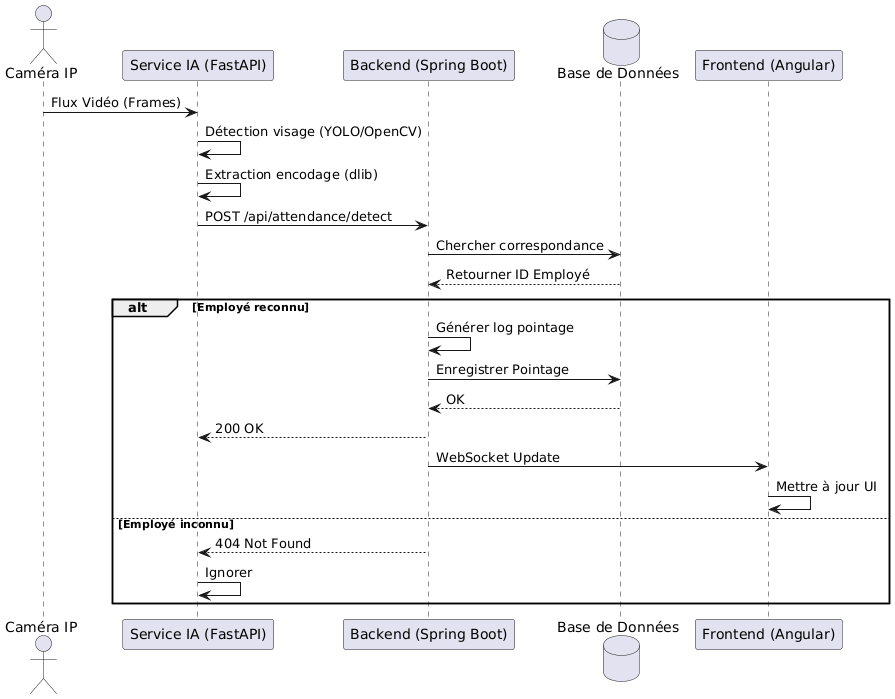
\includegraphics[width=0.9\textwidth]{seq_ai.png}
  \caption{Diagramme de séquence - Reconnaissance Faciale et Pointage Automatique}
  \label{fig:seq_ai}
\end{figure}

\subsection{Diagramme de classes}
La figure \ref{fig:classes} représente la structure des données partagées entre l'application et l'IA.

\begin{figure}[h]
  \centering
  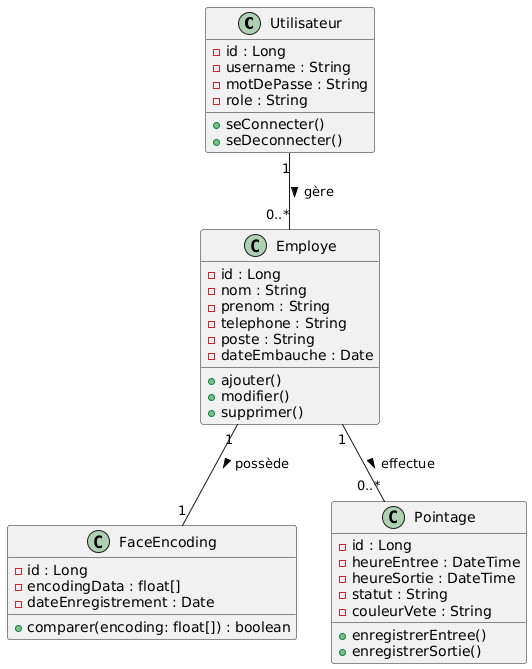
\includegraphics[width=1\textwidth]{class_diagram.png}
  \caption{Diagramme de classes Global Farm AI}
  \label{fig:classes}
\end{figure}

\section{Conclusion}
Ce chapitre a établi l'ensemble des besoins du système et défini son architecture via UML. Le chapitre
suivant présentera les choix technologiques et l'environnement de développement retenus.

% --------------------------------------------------------------
% CHAPITRE 3 : Environnement et Choix Techniques
% --------------------------------------------------------------
\chapter{Environnement et Choix Techniques}

\section{Introduction}
Ce chapitre expose l'environnement matériel et les différentes technologies employées dans la réalisation de la plateforme.

\section{Architecture logicielle}
L'architecture multi-tiers adoptée connecte le flux IA (Python/FastAPI), le serveur central
(Java/Spring Boot) et l'interface web (Angular) via des API RESTful.

\section{Environnement matériel et outils de développement}

\subsection{Environnement matériel}
Le développement a été effectué sur des PC performants capables de traiter des flux vidéo pour le modèle IA.

\subsection{Outils de développement}
L'utilisation de VS Code, IntelliJ IDEA et Git a permis de structurer efficacement le travail.

\section{Technologies de l'intelligence artificielle (service Python)}

\subsection{Python et FastAPI}
Python a été privilégié pour sa grande variété de bibliothèques d'IA, et FastAPI pour l'exposition ultra-rapide des résultats sous forme d'API REST.

\subsection{OpenCV et modèles de Computer Vision}
OpenCV gère la capture et la manipulation des frames, tandis que dlib permet l'encodage précis des visages. YOLO est utilisé pour la détection de personnes et des vêtements.

\section{Technologies Backend (serveur Java)}

\subsection{Java et Spring Boot}
Le socle applicatif principal garantit la sécurité avec Spring Security et JWT.

\subsection{Base de données PostgreSQL}
Une base de données relationnelle robuste pour la sauvegarde de l'historique de présences.

\subsection{Communication API RESTful}
La standardisation JSON a permis une grande interopérabilité entre Angular, Spring Boot et Python.

\section{Technologies Frontend (application web)}

\subsection{Framework Angular et TypeScript}
Le framework côté client garantit une application mono-page (SPA) réactive.

\subsection{SCSS et Design System}
Le design adopté intègre des thèmes sombres et une approche Glassmorphism pour le rendu cyber-technologique.

\section{Conclusion}
Ce chapitre a justifié l'ensemble des choix techniques effectués. Le chapitre suivant présentera la
réalisation concrète et les résultats des tests de validation.

% --------------------------------------------------------------
% CHAPITRE 4 : Réalisation et Tests
% --------------------------------------------------------------
\chapter{Réalisation et Tests}

\section{Introduction}
Cette dernière étape permet de visualiser les interfaces développées et d'analyser les résultats des tests de l'IA.

\section{Réalisation des interfaces utilisateurs}

\subsection{Interface d'authentification}
Conception d'une interface de connexion moderne (thème sombre, animations cybernétiques).

% \begin{figure}[h]
%   \centering
%   \includegraphics[width=0.85\textwidth]{login.png}
%   \caption{Interface d'authentification de Farm AI}
%   \label{fig:login}
% \end{figure}

\subsection{Tableau de bord analytique (Dashboard)}
Visualisation des présences, de l'historique et de la timeline des activités.

% \begin{figure}[h]
%   \centering
%   \includegraphics[width=0.85\textwidth]{dashboard.png}
%   \caption{Tableau de bord analytique de la plateforme}
%   \label{fig:dashboard}
% \end{figure}

\subsection{Interface de configuration de l'IA et flux vidéo}
Intégration du flux caméra en temps réel avec détection superposée.

\section{Intégration du système IA avec le Backend}
La communication entre le script Python (\texttt{camera\_ai\_stream.py}) et le backend Spring Boot
repose sur des appels HTTP POST transmettant les informations de détection (identifiant employé,
horodatage, attributs vestimentaires) au format JSON.

\section{Tests et validation}

\subsection{Tests de précision de l'IA}
Nous avons testé les performances des différents modèles sous diverses conditions d'éclairage.

\begin{table}[h]
  \centering
  \begin{tabular}{lccc}
    \toprule
    \textbf{Modèle} & \textbf{Précision (\%)} & \textbf{Rappel (\%)} & \textbf{F1-Score} \\
    \midrule
    dlib ResNet & 94,5 & 92,0 & 0,932 \\
    FaceNet     & 97,2 & 95,8 & 0,965 \\
    \bottomrule
  \end{tabular}
  \caption{Tableau 4.1 : Comparaison des performances des modèles de reconnaissance faciale}
  \label{tab:perf}
\end{table}

\subsection{Tests de charge et de performance}
Le service FastAPI s'est avéré très résilient face à plusieurs flux vidéo simultanés.

\subsection{Tests de l'interface utilisateur}
Les interactions sur le tableau de bord Angular sont fluides et réagissent bien aux web-sockets émis par le backend lors des pointages.

\section{Conclusion}
Les tests réalisés confirment la robustesse et la précision du système Farm AI. L'ensemble des
objectifs fixés en début de projet ont été atteints.

% --------------------------------------------------------------
% CONCLUSION GÉNÉRALE ET PERSPECTIVES
% --------------------------------------------------------------
\chapter*{Conclusion générale et Perspectives}
\addcontentsline{toc}{chapter}{Conclusion générale}

Ce projet a permis de concevoir et de développer de bout en bout la plateforme \textit{Farm AI},
un système de gestion agricole intelligent intégrant la reconnaissance faciale en temps réel, le
suivi automatique des présences et un tableau de bord analytique. Les objectifs fonctionnels et
non fonctionnels définis en amont ont été atteints, et les tests de validation ont confirmé la
fiabilité du système.

\textbf{Perspectives d'évolution :}
\begin{itemize}
  \item Intégration de caméras thermiques pour évaluer la santé des employés et des animaux.
  \item Déploiement sur le Cloud (AWS / Azure) avec une architecture Kubernetes.
  \item Ajout d'une application mobile pour les gestionnaires nomades.
  \item Extension du modèle IA pour la détection d'équipements de sécurité (casques, gilets).
\end{itemize}

% --------------------------------------------------------------
% BIBLIOGRAPHIE
% --------------------------------------------------------------
\begin{thebibliography}{9}
\addcontentsline{toc}{chapter}{Bibliographie}

\bibitem{angular}
Documentation officielle Angular.
\textit{Angular Framework}.
[En ligne]. Adresse URL : \url{https://angular.io/}.
(Page consultée le 01 juin 2025.)

\bibitem{opencv}
G.~Bradski et A.~Kaehler.
\textit{Learning OpenCV 3: Computer Vision in C++ with the OpenCV Library}.
O'Reilly Media, Sebastopol, 1\,000~p., 2016.
Documentation en ligne : \url{https://opencv.org/}.

\bibitem{springboot}
Documentation officielle Spring.
\textit{Spring Boot Reference Documentation}.
[En ligne]. Adresse URL : \url{https://spring.io/projects/spring-boot}.
(Page consultée le 01 juin 2025.)

\end{thebibliography}

% --------------------------------------------------------------
% ANNEXES
% --------------------------------------------------------------
\appendix
\chapter*{Annexes}
\addcontentsline{toc}{chapter}{Annexes}

\section*{Annexe 1 : Listing du script Python de traitement vidéo}
\addcontentsline{toc}{section}{Annexe 1 : Listing du script Python}
\textit{Script camera\_ai\_stream.py}

\section*{Annexe 2 : Schéma de la base de données}
\addcontentsline{toc}{section}{Annexe 2 : Schéma de la base de données}
\textit{Schéma entité-association}

\end{document}
